\documentclass[a4paper]{article}

\usepackage[utf8]{inputenc}
\usepackage[T1]{fontenc}
\usepackage{textcomp}
\usepackage[english]{babel}
\usepackage{amsmath, amssymb}
\usepackage{listings}
\usepackage{natbib}
\usepackage{subfig}
% figure support
\usepackage{import}
\usepackage{xifthen}
\pdfminorversion=7
\usepackage{pdfpages}
\usepackage{transparent}
\newcommand{\incfig}[1]{%
	\def\svgwidth{\columnwidth}
	\import{./figures/}{#1.pdf_tex}
}

\pdfsuppresswarningpagegroup=1
\title{Miniproject 2 \\ Classification of handwritten digits using SVD}
\author{Linus Falk}

\begin{document}
\maketitle
\section*{Introduction}
Pattern recognition can be solved with various methods, this project aims to solve the classic recognition of handwritten digits with the use of singular value decomposition or SVD for short. 

\subsection*{Singular value decomposition}
The SVD decomposition or factorization exist for any  a real or complex matrix, rectangular or square. The SVD factorization of a matrix M is presented below:

\begin{equation}
	\begin{aligned}
		M = U \Sigma V^{*}
	\end{aligned}
\end{equation}
Where $U$ and $V^{*}$ are unitary matrices and the columns are sets of orthonormal vectors and can be seen as basis vectors of the column space and row space. These two matrices represent rotation and reflection while $\Sigma$ act as scaling \citep{svd}.

\subsection*{The data set}
The data set to create this model to recognise handwritten digits consists of a training and test  set with pictures of handwritten digits made of 28x28 pixels. These pictures are flatten to a column of 784 numbers representing the gray scale of in the picture. The sets are accompanied by the labels for each digit in the training and test set \citep{note} . Example of digit presented below:

\begin{figure}[ht!]
\centering
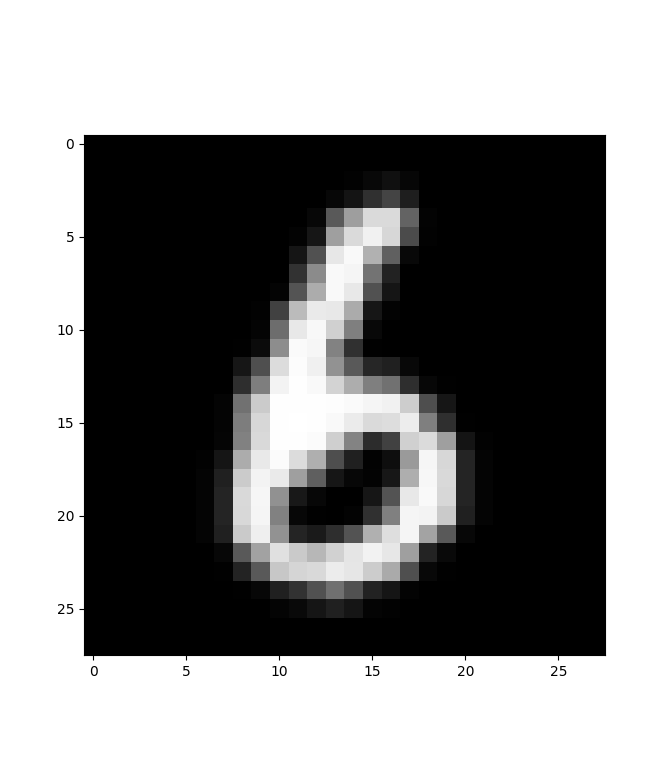
\includegraphics[scale=0.3]{example.png}
\caption{Example of digit}
\label{fig:dig}
\end{figure}


\section*{Method}
The idea is to use the SVD decomposition of ten different matrices of constructed of training digit pixel values: $A_0,A_1,\ldots,A_{9}$ where each columns consists of the 784 pixel values for a digit. Using the SVD of each matrix we obtain the  orthonormal basis for the column space of each A. Then the test images can be represented in terms of these orthonormal basis. Because most of the columns of A are nearly linearly dependent (caused by similarity between the representation of the same digit) we only need a couple of the to represent the digit.
To test the similarity between a test digit and one of theses bases we calculate the following residual:

\begin{equation}
	\begin{aligned}
		\|(I-U^{T}_kU_k)d\|_2
	\end{aligned}
\end{equation}

If the test digit would be a perfect representation captured by the chosen columns of U, the residual would be zero. By testing the test digit with the different U's and compare the residual we can conclude what digit it is most likely to be.  



\begin{figure}[ht]%
    \centering
    \subfloat[\centering $U_0$ with test digit 9]{{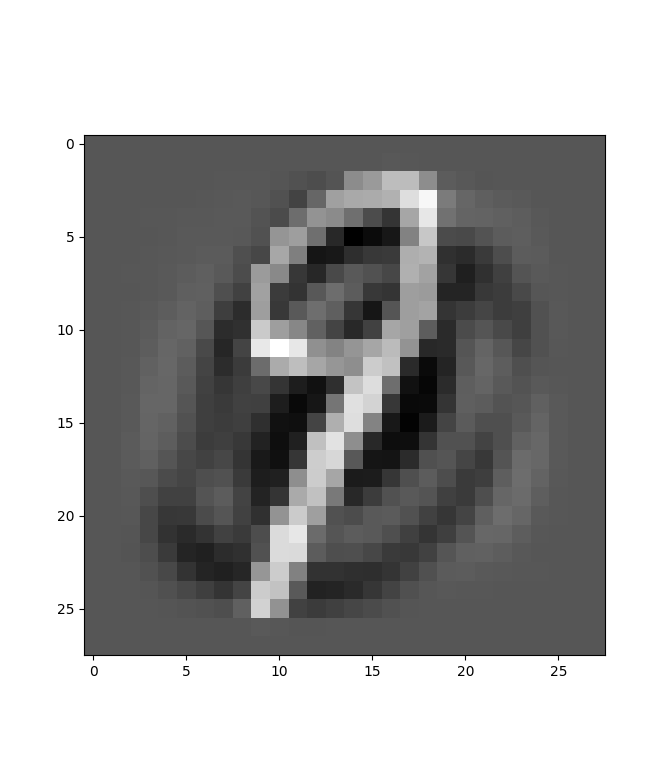
\includegraphics[width=5cm]{U0_T9.png} }}%
    \qquad
    \subfloat[\centering $U_9$ with test digit 9]{{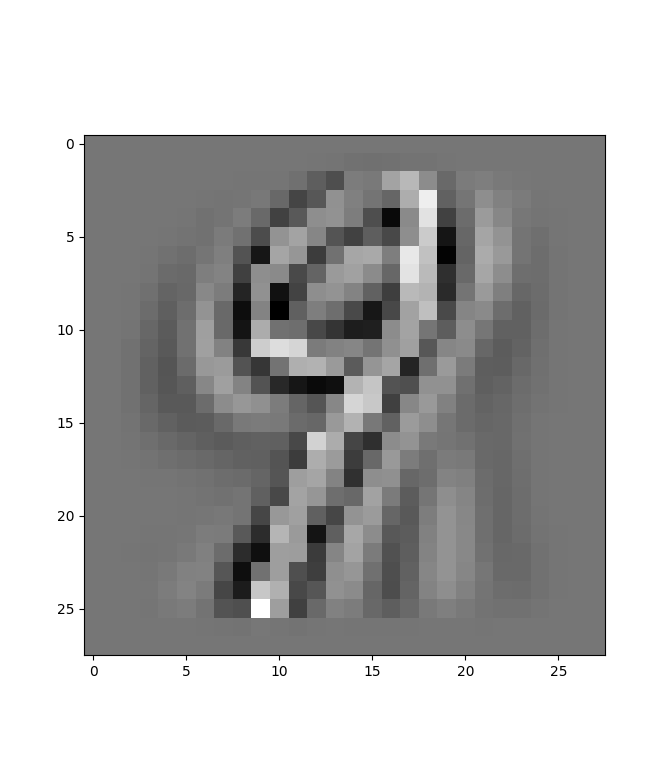
\includegraphics[width=5cm]{U9_T9.png} }}%
    \caption{A digit 9 tested with 20 columns of U for the digit zero and nine}%
    \label{fig:example}%
\end{figure}



\subsection*{Implementation}
The implementation was done using a Python script were the first step was to sort all test digits in a matrix with the same digit: $A_0$ with all zeros and so on. This was done for two cases: 1: with all training digits and 2: with 7500 training digits. The SVD was then calculated for each of these cases and type of digit. Comparing the residuals of a test digit with equation (2) and choosing the one with lowest yielded the predictions that was then checked with the label.  

\begin{lstlisting}[language=Python]
A = [[],[],[],[],[],[],[],[],[],[]]

for j in range(1000):
    A[TrainLabels[0][j]].append(TrainDigits[:, j])

U = []
for i in range(10):
    d = A[i]
    d = np.asarray(d)
    d = d.transpose()
    u, s, vh = np.linalg.svd(d)
    U.append(u)

\end{lstlisting}

Testing different number of columns was done using a reduced number of test digits (200) and a for loop to change the number of columns. 



\begin{lstlisting}[language=Python]

NumerOfTests = 200
for t in range(2,31,1):
    precictions = []
    for i in range(NumerOfTests):
        result = []
        for x in range(10):
            u1 = U[x]
            u1 = u1[:, :t]
            result.append(np.linalg.norm((I - 
	    u1@u1.transpose())@TestDigits[:, i]))

        min_value = min(result)
        min_index = result.index(min_value)
        if min_index == TestLabels[0][i]:
            precictions.append(1)
        else:
            precictions.append(0)

    precentage = (sum(precictions)/NumerOfTests)*100
    print(str(t) + ' ' + str(precentage) + '%')
	
\end{lstlisting}
When the approximation of the optimal number of columns was done was the complete set of test digits tested.

\section*{Result and discussion}
The result of the tests with 200 test digits to establish some guidance to choose how many columns: \textbf{n}  to use is presented below:

\newpage

\begin{table}[ht]
\begin{tabular}{rlrlrlrlrlrl}
\multicolumn{1}{l}{\textbf{n}} & \textbf{acc\%} & \multicolumn{1}{l}{\textbf{n}} & \textbf{} & \multicolumn{1}{l}{\textbf{n}} & \textbf{} & \multicolumn{1}{l}{\textbf{n}} & \textbf{} & \multicolumn{1}{l}{\textbf{n}} & \textbf{} & \multicolumn{1}{l}{\textbf{n}} & \textbf{} \\
\textbf{2}                     & 81.0           & \textbf{7}                     & 91.5      & \textbf{12}                    & 93.0      & \textbf{17}                    & 91.0      & \textbf{22}                    & 90.5      & \textbf{27}                    & 92.5      \\
\textbf{3}                     & 85.5           & \textbf{8}                     & 91.0      & \textbf{13}                    & 92.5      & \textbf{18}                    & 92.0      & \textbf{23}                    & 91.5      & \textbf{28}                    & 92.5      \\
\textbf{4}                     & 84.0           & \textbf{9}                     & 93.0      & \textbf{14}                    & 92.0      & \textbf{19}                    & 92.0      & \textbf{24}                    & 90.5      & \textbf{29}                    & 93.0      \\
\textbf{5}                     & 87.0           & \textbf{10}                     & 92.0      & \textbf{15}                    & 92.5      & \textbf{20}                    & 92.0      & \textbf{25}                    & 92.0      & \textbf{30}                    & 93.5      \\
\textbf{6}                     & 88.0           & \textbf{11}                    & 92.5      & \textbf{16}                    & 92.0      & \textbf{21}                    & 91.5      & \textbf{26}                    & 92.5      & \multicolumn{1}{l}{}           &          
\end{tabular}
\caption{Accuracy, trained with 7500 training digits}
\end{table}

\begin{table}[ht]
\begin{tabular}{rlrlrlrlrlrl}
\multicolumn{1}{l}{\textbf{n}} & \textbf{acc\%} & \multicolumn{1}{l}{\textbf{n}} & \textbf{} & \multicolumn{1}{l}{\textbf{n}} & \textbf{} & \multicolumn{1}{l}{\textbf{n}} & \textbf{} & \multicolumn{1}{l}{\textbf{n}} & \textbf{} & \multicolumn{1}{l}{\textbf{n}} & \textbf{} \\
\textbf{2}                     & 80.0           & \textbf{7}                     & 91.0      & \textbf{12}                    & 92.5      & \textbf{17}                    & 91.0      & \textbf{22}                    & 91.0      & \textbf{27}                    & 92.5      \\
\textbf{3}                     & 86.0           & \textbf{8}                     & 90.0      & \textbf{13}                    & 92.5      & \textbf{18}                    & 91.5      & \textbf{23}                    & 91.5      & \textbf{28}                    & 92.0      \\
\textbf{4}                     & 87.0           & \textbf{9}                     & 92.0      & \textbf{14}                    & 91.5      & \textbf{19}                    & 91.5      & \textbf{24}                    & 92.5      & \textbf{29}                    & 92.0      \\
\textbf{5}                     & 87.0           & \textbf{10}                    & 91.5      & \textbf{15}                    & 92.5      & \textbf{20}                    & 92.0      & \textbf{25}                    & 93.5      & \textbf{30}                    & 92.0      \\
\textbf{6}                     & 89.5           & \textbf{11}                    & 93.0      & \textbf{16}                    & 92.0      & \textbf{21}                    & 91.5      & \textbf{26}                    & 93.0      & \multicolumn{1}{l}{}           &          
\end{tabular}
\caption{Accuracy: trained with all training digits}
\end{table}

The number of columns didn't seem to affect the result except with very few, $<8$. Increasing the number of training digits didn't improve the result either. The final test was therefore done with 7500 training digits to construct the U's and  20 columns of these. The number of columns select was  something in the middle of the tested span of $>10$ columns. This resulted in an accuracy of: \textbf{95.44\%}. The result show that the SVD is a powerful tool in data analysis and can be used for simpler image recognition tasks.  

\bibliographystyle{unsrt}
\bibliography{references}
\end{document}
